% !TEX root = RailVehicleIntroduction.tex
\section{Train dynamics}
\subsection{Introduction}

\frame{\frametitle{Coordinate system and forces}
\framesubtitle{}
\begin{columns}[t] 
     \begin{column}[T]{6cm} 
     \begin{itemize}
		\item Coordinates
     	\begin{itemize}
     		\item $x$ positive in direction of travel
		\item $z$ to the top
		\item $y$ to form Cartesian system
     	\end{itemize}
	\item Forces acting:
	\begin{itemize}
		\item Resistances
		\begin{itemize}
		\item Train-, Track resistance
		\end{itemize}
		\item Traction
		\item Braking force
		\end{itemize}
	\end{itemize}
     \end{column}
     	\begin{column}[T]{6cm} 
         	\begin{center}
            		\begin{tikzpicture}[scale=3.5,tdplot_main_coords]
    \coordinate (O) at (0,0,0);
    \tdplotsetcoord{P}{1}{70}{70}

\draw[thick,->] (0.1,0.4,0.1) -- (-.8,.4,0.1) node[anchor=south west]{$y$};
\draw[thick,->] (0.1,0.4,0.1) -- (0.1,1.2,0.1) node[anchor=south west]{$x$};
\draw[thick,->] (0.1,0.4,0.1) -- (0.1,.4,.5) node[anchor=south]{$z$};

\draw[thick] (-0.1,-.5,-0.1) -- (-0.1,1.2,-.1);
\draw[thick] (0.1,-.5,-0.1) -- (0.1,1.2,-.1);

    \draw[fill=blue!80!black,fill opacity=0.5] (O) -- (Py) -- (Pyz) -- (Pz) -- cycle;
    \draw[fill=blue!80!black,fill opacity=0.5] (O) -- (Px) -- (Pxy) -- (Py) -- cycle;
    \draw[fill=blue!80!black,fill opacity=0.5] (O) -- (Px) -- (Pxz) -- (Pz) -- cycle;
    \draw[fill=blue!80!black,fill opacity=0.5] (Pz) -- (Pyz) -- (P) -- (Pxz) -- cycle;
    \draw[fill=blue!80!black,fill opacity=0.5] (Px) -- (Pxy) -- (P) -- (Pxz) -- cycle;
    \draw[fill=blue!80!black,fill opacity=0.5] (Py) -- (Pxy) -- (P) -- (Pyz) -- cycle;
  \end{tikzpicture}
        		\end{center}
     \end{column}
 \end{columns}
}


\frame{\frametitle{Forces acting on the vehicle}
\begin{center}
\vspace{1cm}
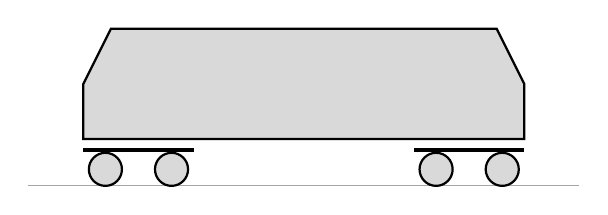
\begin{tikzpicture}[scale = 0.7]
\draw[draw = gray!70] (-1, -.85) -- (9, -.85);
\draw[thick, fill = gray!30] (0,0) -- (0,1) -- (.5,2) -- (7.5,2) -- (8,1) -- (8,0) -- cycle;
\draw[ultra thick] (0, -.2) -- (2, -.2); 
\draw[thick, fill = gray!30] (.4, -.55) circle (.3);
\draw[thick, fill = gray!30] (1.6, -.55) circle (.3);
\begin{scope} [shift = {(6,0)}]
\draw[ultra thick] (0, -.2) -- (2, -.2); 
\draw[thick, fill = gray!30] (.4, -.55) circle (.3);
\draw[thick, fill = gray!30] (1.6, -.55) circle (.3);
\end{scope}
\end{tikzpicture}
\end{center}
}


\subsection{Train and track resistances}
\frame{\frametitle{Train and track resistances}

\begin{columns}[t] 
     \begin{column}[T]{6cm} 
     \begin{itemize}
		\item Track resistances
     	\begin{itemize}
     		\item Grade resistance
			\item Curve resistance
			\item Switch resistance
     	\end{itemize}
	\item Train resistances
	\begin{itemize}
		\item Rolling resistance ($\propto 1$)
		\begin{itemize}
		\item Wheel deformation
		\end{itemize}
		\item Bearing resistance ($\propto 1$)
		\begin{itemize}
		\item Axle box friction
		\end{itemize}
		\item Dynamical resistance ($\propto v$)
		\begin{itemize}
		\item From hunting motion
		\end{itemize}
		\item Aerodynamical drag ($\propto v^2$)
		\end{itemize}
	\end{itemize}
     \end{column}
     	\begin{column}[T]{6cm} 
		Common equations:\\
		\small Strahl formula (suitable for freight trains):
		\begin{equation}
		\label{Eq:Strahl}
			f_{WW} = 1{,}6 \permil +  5{,}7 \permil \left( \frac{v}{100 \frac{\mathrm{km}}{\mathrm{h}}} \right)^2
		\end{equation}
		Sauthoff formula (suitable for passenger trains ($n_C$ coaches, $m_T$ train mass)):
		\begin{equation}
		\label{Eq:Sauthoff}
		\begin{split}
			f_{WW} &= 1{,}6 \permil + 0{,}25 \permil \left( \frac{v}{100 \frac{\mathrm{km}}{\mathrm{h}}} \right) \\
			&+ \frac{683 \, \mathrm{N}(2{,}7 + n_{C}) }{m_{T} g} \left( \frac{v+ 12 \frac{\mathrm{km}}{\mathrm{h}}}{100 \frac{\mathrm{km}}{\mathrm{h}}} \right)^2
		\end{split}
		\end{equation}
      \end{column}
 \end{columns}
}


\subsection{Braking of trains}
\frame{\frametitle{Braking of trains}
\begin{center}
\includegraphics[width=10.0cm]{3CarTrainset.png}
\end{center}

}


\subsection{Wheel-Rail Contact}
\frame{\frametitle{Wheel-Rail Normal Contact}
\begin{center}
\begin{tikzpicture}[scale = .7]
\draw[thick, pattern = north west lines, 
rounded corners = 2pt
] (-1,0) -- (-2,0) -- (-2, .15) -- (-1.6, .25) -- (-1.6, .7) -- (-1.9, .75) -- (-1.9, .95) to[out = 10, in = 170] 
(-1.1, .95) -- (-1.1, .75) -- (-1.4, .7) --(-1.4, .25) -- (-1,.15) -- cycle;
\draw[thick, pattern = north east lines,
rounded corners = 2 pt] (-2.5, 1.3) -- (-2.5, .8) 
to[out = 270, in = 270] (-2.2,.8) -- (-2.2, .9)  -- (-.9, 1.1) -- (-.9, 1.3); 
\draw[thick, fill = gray!70, opacity = 0.9] (2.5, 3) circle (2.1 cm);
\draw[thick, fill = gray!80] (2.5, 3) circle (2 cm);
\draw[thick, fill = gray!10] (2.5, 3) circle (1.8 cm);
\draw[thick, fill = black!90] (2.5, 3) circle (.2 cm);
\shade[top color = gray!80, bottom color = gray!20] (0,0) rectangle (5,1);
\draw (0,1) -- (5,1);
\draw (0,.8) -- (5,.8);
\draw (0,.1) -- (5,.1);
\draw[thick] (0,0) -- (5,0);
\draw[-angle 90, line width = 0.1cm, draw = red!8!green!47!blue!60] (5.5,2) to[out = 0, in = 100] (10,-2);
\draw (10, -4) ellipse (2.5cm and 1.5cm);
\end{tikzpicture}
\end{center} 
}

\frame{\frametitle{Wheel-Rail Tangential Contact}
\begin{center}
\begin{tikzpicture}[scale = .6]
\draw[thick, fill = gray!70, opacity = 0.9] (2.5, 3) circle (2.1 cm);
\draw[thick, fill = gray!20] (2.5, 3) circle (2 cm);
\draw[thick, fill = black!90] (2.5, 3) circle (.2 cm);
\foreach \alpha in {0, 20,...,320} {
\draw (2.5,3) -- +(\alpha-70:2cm);
}
\foreach \alpha in {320, 325,...,355} {
\draw (2.5,3) to +(\alpha-70:1.3cm) to[out = \alpha-70, in = \alpha/320*\alpha+110] +(\alpha-70:2cm);
}
\draw[thick, draw = blue!80!black, -angle 90] (3.5, 3) arc (0:180:1cm); 
\node at (2.5,4.3) {$T$};
\begin{scope}[shift = {(0,.1)}]
\shade[top color = gray!80, bottom color = gray!20] (0,0) rectangle (5,1);
\draw (0,1) -- (5,1);
\draw (0,.8) -- (5,.8);
\draw (0,.1) -- (5,.1);
\draw[thick] (0,0) -- (5,0);
\end{scope}
\draw[-angle 90, line width = 0.1cm, draw = red!8!green!47!blue!60] (5.5,3) %to[out = 0, in = 100] 
-- (7,3);
\draw[fill = gray!30, draw = gray!30] (10, 3) ellipse (2.5cm and 1.5cm);
\node at (11.5,3) {Slip};
\draw[fill = gray!70, draw = gray!70] (9, 3) ellipse (1.5cm and 1.2cm);
\node at (9,3) {Stick}; 
\draw[-angle 90, line width = 0.1cm, draw = red!8!green!47!blue!60] (10,1) %to[out = 0, in = 100] 
-- (10,-1);
\draw[->] (5, -6.5) -- (5,-2) node[pos = 0.9, above, rotate = 90] {Friction $\mu$}; 
\draw[->] (5, -6.5) -- (12,-6.5) node[pos = 0.9, below] {Creep $s$}; 
\end{tikzpicture}
\end{center} 
}
